\chapter{Tutamen: Next-Generation Secret Storage}
\label{chap:tutamen}

While Custos (Chapter~\ref{chap:custos}) provides a sound
first-generated secret storage system, it has a number of flaws that
make solving some of the more nuanced secret storage challenges
difficult. Tutamen is a secret storage system design to overcome these
challenges. Tutamen applies the lessons learned from building Custos
to create a next-generation secret storage system with native support
for multi-provider secret sharding and automated secret access.

\section{A New Approach}
\label{chap:tutamen:new}

Tutamen aims to correct flaws in previous SSaaS systems such a Custos
and relates first generation secret storage systems such as
Vault~\cite{vault}. In particular, Tutamen aims to provide better
support for multi-SSP sharding, for autonomous use cases, and for
global-scale scenarios that extended beyond a single administrative
domain.

\subsection{Flaws in Custos}

Custos has two main flaws, the correction of which informs the Tutamen
design. Namely:

\begin{packed_item}
\item The Custos access control chain and permissioning system is
  quite complex. This makes it difficult to properly reason about the
  net effect of an access control rule or how best to apply that rule
  in an automated or distributed fashion.
\item Custos lacks primitives for easing the synchronization of secret
  shards across multiple Custos servers. While it is possible to use
  Custos in a multi-provider manner, the lack of supporting primitives
  makes doing so more complex than it needs to be.
\end{packed_item}

Tutamen aims to correct these flaws. On the access control front, the
true benefit of Custos' access control system is its ability to
support out-of-band (i.e. ``implicit'' attributes) authentication
attributes (e.g. IP address, etc). Custos's ``explicit'' attributes
(e.g. user-provided passwords, etc) can be better represented via
cryptographic authentication practices such as the use of client TLS
certificates. Cryptographic methods are both stronger and more
convenient then requiring users to provide usernames, passwords, or
other shared secrets. Thus, Tutamen replaces all of Custos's in-band
(i.e. ``explicit'') attributes with cryptographically secure TLS
client authentication mechanisms. Tutamen then merges Custos's
out-of-band (``implicit'') attributes into a general purpose (and
optional) out-of-band authentication mechanism capable of verifying a
range of out-of-band parameters from request attributes such as time
and IP address to multi-factor options such as SMS text message or
email. Like Custos, this out-of-band system is extensible and
plugin-based. Tutamen thus captures the best of the Custos access
control design while also reducing complexity and increasing security.

On the multi-server front, Tutamen adds support for primitives that
make it easier to shard Tutamen secrets across multiple servers. Most
notably, Tutamen allows clients to request specific secret IDs when
storing secrets. This allows a client to reuse a single secret ID
across multiple servers and simplifies the mapping of a logically
singular secret to multiple shards. Tutamen also separates the secret
storage and access control components of the SSaaS model into separate
servers, further allowing the user additional flexibility in
distributing secret storage duties across multiple providers.

These techniques are discussed in more detail in
Section~\ref{chap:tutamen:arch}.

\subsection{The Ideal Secret Storage System}

As discussed in Chapter~\ref{chap:ssaas}, unlike standard
configuration management systems or specific secret storage systems
such as password managers, a general purpose secret storage presents a
number of unique requirements. Such a system must be capable of
satisfying the following capabilities:

\begin{packed_item}
\item Store a wide-range of arbitrary secret data in a secure manner
\item Enforce fine-grained access control requirements
\item Support a range of authentication sources/methods
\item Provide audit logs tracking secret access history
\end{packed_item}

Since the development of Custos, a number of general purpose secret
storage systems have been deployed by industry, including HashiCorp's
Vault~\cite{vault}, Lyft's Confidant~\cite{confidant}, and Square's
Keywhiz~\cite{keywhiz}. These systems exist to fulfill some or all of
the requirements listed above. Such systems, however, are hindered by
several key limitations. First, they generally require at least one
highly trusted server as the basis of their security model, making
them unsuitable for operation atop untrusted infrastructure. Second,
they tend to lack support for use cases requiring autonomous or remote
access to secret material in a secure manner. And finally, they do not
scale well beyond a single administrative domain. These deficiencies
give rise to two more secret storage requirements:

\begin{packed_item}
\item Avoidance of the need to place a high degree of trust in any
  single system outside the application that wishes to store a secret.
\item Ability to support a range of secret access use cases, including
  use cases where automatic or remote access to secrets is required,
  or where data must be accessible beyond a single administrative
  domain.
\end{packed_item}

It is toward these final two requirements that Tutamen attempts to
advance the state of the art over existing secret storage systems. In
particular, Tutamen supports operational modes where no single entity
other than the application must be trusted. This allows users to
leverage third party secret storage providers running Tutamen servers
without having to place high degrees of trust in any single provider
(see Chapter~\ref{chap:trust}). Like Custos, Tutamen also provides
support for a modular authentication interface. This interface makes
Tutamen suitable for use in situations where it is desirable to
leverage external environmental information to automatically evaluate
the authenticity of a secret request or where it is necessary to keep
a human in the authentication loop without actually requiring that the
human be physically present. For example, Tutamen can be used to store
the disk encryption keys required to boot a headless server, and only
release these keys to the server requesting them when a human responds
to a text message confirming the boot request. Finally, Tutamen is
designed to support collaboration between loosely-organized users and
does not aim to limit its scope to within a single administrative
domain.

\section{Tutamen Architecture}
\label{chap:tutamen:arch}

The Tutamen SSaaS platform is designed to handle the storage of
arbitrary secret material from a range of applications. To accomplish
this, Tutamen employees three discrete architectural components:

\begin{packed_desc}
\item[Access Control Servers (ACS):] The systems responsible for
  storing and enforcing secret access control requirements and for
  authenticating secret requests.
\item[Storage Servers (SS):] The systems responsible for storing
  secrets (or parts of secrets).
\item[Applications:] The systems leveraging the Tutamen platform to
  store and retrieve secrets.
\end{packed_desc}

The bulk of all Tutamen communication occurs between an application
and one or more of each type of server. Inter-server communication is
kept to a minimum to support scalability. All communication in Tutamen
takes place via TLS/HTTPS~\cite{dierks2008} connections, and in some
cases leverages mutual TLS to provide both client and server
authentication. Both access control and storage servers are designed
to be used individually or in sets. E.g., an application may store its
secrets on a single storage server and delegate access control to a
single access control server, or the application may shard its secrets
across multiple storage servers and delegate access control to
multiple access control servers, or any combination thereof.

\subsection{Access Control Servers}
\label{chap:tutamen:arch:acs}

Tutamen access control servers (ACS) are responsible for
authenticating Tutamen requests as well as storing and enforcing all
Tutamen access control requirements. Access control servers expose a
number of core data structures that reflect the manner in which they
operate. Figure~\ref{fig:tutamen:acstructs} shows these structures.

\begin{figure}[t]
  \centering
  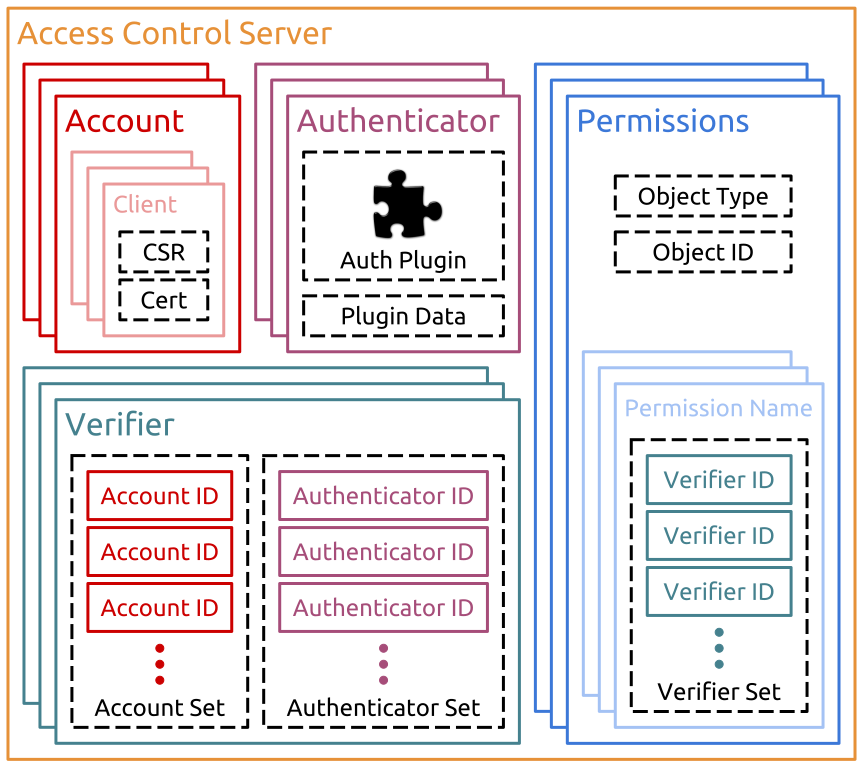
\includegraphics[width=0.48\textwidth]{./figs/out/Tutamen-Structs-ACS.pdf}
  \caption{Access Control Server Data Structures}
  \label{fig:tutamen:acstructs}
\end{figure}

In order to track and control access from specific actors, the access
control server uses per-actor accounts. These accounts are generally
designed to map to individual end users, but they can be used to track
any entity to which one wishes to assign specific access control
privileges. Accounts thus form the basis of controlling and sharing
access to secrets via Tutamen. Within each account are one or more
clients. While accounts represent logically singular entities, clients
represent specific devices controlled by such entities. Each account
has one or more clients. For example, Jane Coworker may have a single
account with three clients: one for her laptop, one for her desktop,
and one for her phone.

Each client is associated with a single x509~\cite{rfc5280} TLS
key/cert-pair used to authenticate the client to the access control
server. The access control server acts as the Certificate Authority
(CA) administering these certificates. When a new client is created it
generates a local private key and uses this key to generate an X509
Certificate Signing Request (CSR). This request is then sent to the
access control server where it awaits approval from an existing client
in the account. If approved, the CSR is used to generate a signed
certificate that is sent back to the new client for use in future ACS
communication. To facilitate bootstrapping new accounts, client CSRs
are also generated and sent to the AC server during new account
creation process. These CSRs are automatically approved and associated
with the new account -- i.e., the initial client is created in tandem
with a new account while all subsequent clients are approved by
previously approved clients.

In addition to accounts, the Tutamen access control server also uses
``authenticators''. Authenticators are modular mechanisms used to
implement contextual access control requirements~\cite{hulsebosch2005}
such as only allowing access during specific times of day or from
specific IP addresses. Authenticators can also be used to implement
multi-factor and/or out-of-band authentication mechanisms such as
confirming approval for a specific request from a user via text
message, or otherwise interfacing with external services to gain
approval.

Accounts and authenticators are combined via verifiers. A verifier
consists of a set of accounts and a set of authenticators. In order to
satisfy a verifier, a request must originate from a client associated
with one of the member accounts and must satisfy all of the member
authenticators. A verifier may contain no authenticators, in which
case authorization is granted solely on the basis of accounts.

The final component of the Tutamen access control server is the
permissions group. Each permissions group corresponds to a specific
object (identified via the combination of an object type and an object
ID) within the Tutamen ecosystem. A permissions group contains one or
more permissions, each corresponding to a specific class of actions
that can be performed on the corresponding object. Each permission is
associated with a set of verifiers. In order to be granted a given
permission, a request must satisfy at least one of the verifiers in
this set.

\subsection{Storage Servers}
\label{chap:tutamen:arch:ss}

Tutamen storage servers (SS) are responsible for storing all or part
of each Tutamen secret. Figure~\ref{fig:tutamen:storagestructs} shows
the core storage server data structures.

\begin{figure}[t]
  \centering
  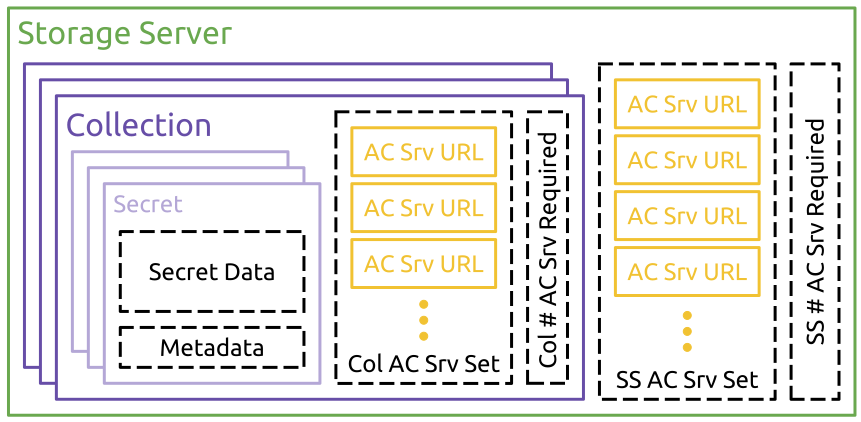
\includegraphics[width=0.48\textwidth]{./figs/out/Tutamen-Structs-SS.pdf}
  \caption{Storage Server Data Structures}
  \label{fig:tutamen:storagestructs}
\end{figure}

The top-level data structure employed by storage servers is the
``collection''. A collection represents a logical grouping of one or
more secrets (or parts of secrets). Associated with each collection is
a list of one or more access control servers delegated with enforcing
the access control requirements for the collection. Access control
granularity is thus set at the per-collection, not per-secret level. A
collection is also capable of storing user-provided metadata to aid in
the mapping of collections to the objects for which they store
secrets.

Each collection stores one or more secrets or secret shards. These
secrets consist of the actual secret data the applications leveraging
Tutamen wishes to store as well as any associated user-provided
metadata. Since access control is set at the per-collection level,
secrets inherit the access control characteristics of the
corresponding collection.

How best to map secret data to collections is left up to each
application. This decision is primarily driven by the fact that access
control is performed on the per-collection level. Thus, if an
application requires that a set of secrets always have a common set of
access control requirements (e.g., per-sector encryption keys for an
encrypted block device), it becomes efficient to group these secrets
into a single collection. Doing so minimizes the complexity of trying
to keep access control requirements synced across multiple secrets,
and increases performance by minimizing the number of requests that
the applications must make to secure tokens from the access control
server. In cases where each secret requires its own access control
requirements (e.g., per-file encryption keys), it is appropriate for
the corresponding application to store only a single secret per
collection.

\subsection{Access Control Protocol}
\label{chap:tutamen:arch:acp}

Access control servers control access related to both internal (i.e.,
access control server) and external (i.e., storage server) objects by
providing signed authorization tokens in response to valid
requests. Similar to previously proposed distributed and federated
access control systems~\cite{calero2010, leandro2012}, each
authorization token grants the bearer a specific permission related to
a specific object. Unlike previous systems, however, Tutamen is
designed to avoid needing to trust any single access control provider
(see \S~\ref{chap:tutamen:arch:distributed}).
Figure~\ref{fig:tutamen:systembase} shows the basic communication
involved in the Tutamen access control process.

\begin{figure}[t]
  \centering
  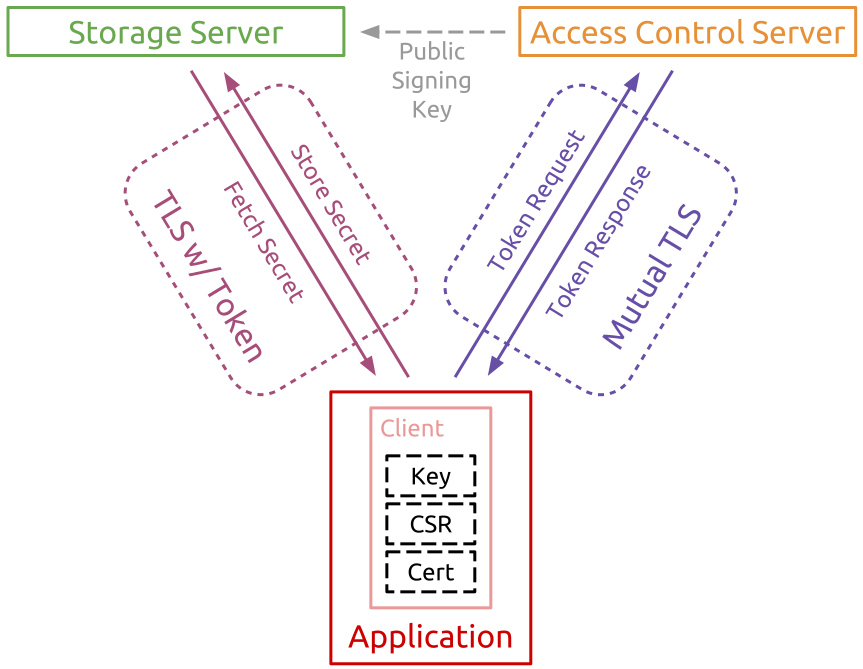
\includegraphics[width=0.48\textwidth]{./figs/out/Tutamen-System-Base.pdf}
  \caption{Access Control Communication}
  \label{fig:tutamen:systembase}
\end{figure}

Each access control server generates authorization tokens in response
to a client sending an authorization request. Each authorization
request (and each corresponding token) includes two claims binding it
to a specific object: the object type and the object ID. Each token
request also contains a claim that binds it to a specific permission
(e.g., read, write, delete, modify) for the corresponding
object. Authorization requests are further bound to the specific
client making the request (authenticated via mutual-TLS), and to an
expiration time after which the token is no longer valid.

Upon receiving an authorization request from a client, the access
control server looks up the permission group for the corresponding
object (identified via the combination of object type and object ID)
and then loads the verifier set corresponding to the requested
permission. The server traverses each verifier in this set, verifying
both client membership in one of the accounts listed in the verifier
as well as executing any authenticator modules required by the
verifier until it finds (or fails to find) a verifier that is
satisfied by the request. If the server is able to verify compliance
with at least one verifier, it grants the authorization request and
returns a signed authorization token that includes the object type,
object ID, granted permission, and expiration time. The bearer of this
token can then present it in conjunction with a request to either the
access control server or a storage server in order to be granted the
right to perform an approved action on the corresponding object.

Other than the bootstrapping operations and the token request
operations themselves, all requests to either storage or access
control servers must be accompanied by a valid token. The receiving
server validates this token using the public signing key of the
associated AC server. For requests to the AC sever itself, this key is
available internally. For requests to external storage servers, the
signing key is downloaded by the storage server from the access
control server and cached for future use. In this manner, access
control servers are responsible both for granting and verifying
authorization requests and signing the corresponding tokens, as well
as for verifying tokens accompanying requests to perform actions on
ACS objects (e.g., to create or modify verifiers or accounts). Storage
servers are responsible only for verifying tokens accompanying
requests to perform actions on SS objects (e.g., to create a
collection or read a secret).

\subsection{Distributed Usage}
\label{chap:tutamen:arch:distributed}

Tutamen is designed to be used in either centralized or distributed
use cases. The simplest Tutamen arrangement (e.g., as shown in
Figure~\ref{fig:tutamen:systembase}) involves leveraging a single
Tutamen access control server and a single storage server. In this
arrangement, the storage server stores a complete copy of each secret
while a sole access control server is charged with enforcing access to
these secrets. While this use case is easy to deploy, it has two
notable downsides. First, it forces the user to place a high degree of
trust in the operator of the access control server (who has complete
control over whether or not the access control rules for a given
secret are being faithfully enforced), as well as in the operator of
the storage server (who, likewise, must faithfully verify incoming
tokens and avoid otherwise leaking secret data). Second, it lacks any
form of redundancy -- if either the access control server or the
storage server is unavailable, applications will be unable to retrieve
any secrets.

As discussed in Chapter~\ref{chap:background}, researchers have
proposed a variety of systems with the goal of minimizing trust
requirements for cloud infrastructure~\cite{bessani2011,
  kallahalla2003, kubiatowicz2000, mahajan2011,
  wilcox-o'hearn2008}. Tutamen applies similar ``minimal-trust'' goals
to the secret storage problem by offering support for a distributed
operation mode as an alternative to single-server operation. Operating
Tutamen in a distributed manner is largely a task that is pushed down
to the application (or client library). With the exception of offering
the necessary primitives to support such operation, both Tutamen
storage and access control servers are designed to be largely agnostic
as to whether they are being used in a centralized or a distributed
manner. This design has the benefit of avoiding server-side scaling
challenges, allowing the extra overhead required for distributed
operation to be supported by each application that requires it.

\begin{figure}[t]
  \centering
  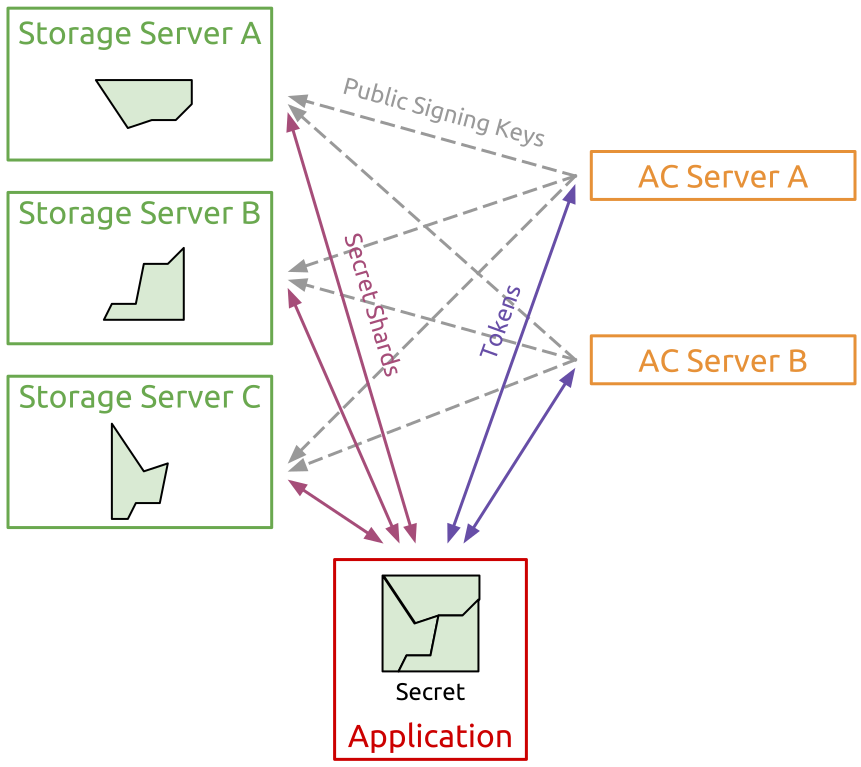
\includegraphics[width=0.48\textwidth]{./figs/out/Tutamen-System-Distributed.pdf}
  \caption{Distributed Operation}
  \label{fig:tutamen:systemdistributed}
\end{figure}

Figure~\ref{fig:tutamen:systemdistributed} shows the basic layout of a
distributed Tutamen setup. As discussed in
Section~\ref{chap:trust:ssaas}, the Tutamen application first shards
its secret using a $(k, n)$ threshold scheme~\cite{krawczyk1993,
  shamir1979}. The application chooses the value of $n$ based on the
number of storage servers it wishes to utilize. The value of $k$ is
then chosen to control how many of the servers must be responsive in
order to retrieve the secret; i.e., the difference between $n$ and $k$
controls how much storage redundancy the system has by dictating the
number of storage servers that can be unavailable before access to the
secret itself is lost. The application then pushes each shard to the
$n$ storage servers. If the application is merely concerned about
storage redundancy, or about their ability to trust a storage server
operator, it can delegate the access control for each secret shard to
a single access control server. To retrieve such a secret the
application would request the necessary token from the access control
server and include it in its request to each storage server for their
respective shard of the secret. When the application receives a
response from $k$ of the storage servers, it is able to reconstruct
the original secret.

In most cases, however, in addition to wishing to mitigate storage
server trust and reliability failures, the application will also wish
to protect itself against access control server trust and reliability
failures. This is accomplished via storage server support for the
specification of two pieces of access control metadata corresponding
to each stored collection: a list of AC servers approved to provide
access control tokens for the collection and a minimum number of
servers from which valid tokens must be received. These parameters
form the basis of a novel, yet simple $(k, n)$ threshold scheme for
access control servers -- e.g., a collection may delegate a list of
$n$ access control servers from which an application must acquire at
least $k$ valid tokens in order to gain access. Thus, if the user does
not wish to trust a single access control server, they may require
tokens from at least $k$ different AC servers in order to access the
data stored in a given collection. As in the storage case, if the
application wishes to withstand the failure of one or more AC servers,
it can specify $n$ possible AC servers where $n > k$.

In order to facilitate ease of management when operating in a
distributed mode, Tutamen supports allowing applications to request
specific UUIDs~\cite{leach2005} for each object they create. This
allows clients to use the same object ID across multiple servers,
alleviating the burden of maintaining a mapping between object IDs and
the servers to which they correspond. Using the same object IDs across
multiple servers also allows for more efficient token management --
e.g., if an application uses the same collection ID on three separate
storage serves, all of which delegate a common set of access control
servers, it is possible (and desirable) for the application to use a
single token granting access to the relevant collection ID on all
three servers. Without this capability, an application would be forced
to request multiple tokens from each access control server
corresponding to the differing collection ID used on each storage
server.\footnote{The ability to request specific object IDs does have
  one downside: it opens Tutamen up to a possible denial-of-service
  (DoS) attack where an attacker attempts to request the object IDs
  they know another application wishes to use for themselves. Since
  each server may only use each object ID once, the first application
  to request a given UUID gets it. Thus, if an adversary knew which
  object IDs a given application planned to use, they could request
  these object IDs on a set of AC servers for themselves, depriving
  the original application of the ability to use those
  servers. Nonetheless, the convenience afforded by allowing
  applications to request specific object IDs outweighs the potential
  for DoS abuse. It is also likely at DoS abuse issues can be
  discouraged via finical incentives - e.g., by charging users for
  each unique UUID.}

\subsection{Usage Example}
\label{chap:tutamen:arch:example}

\begin{figure}[!t]
  \centering
  \begin{subfigure}[t]{0.48\textwidth}
    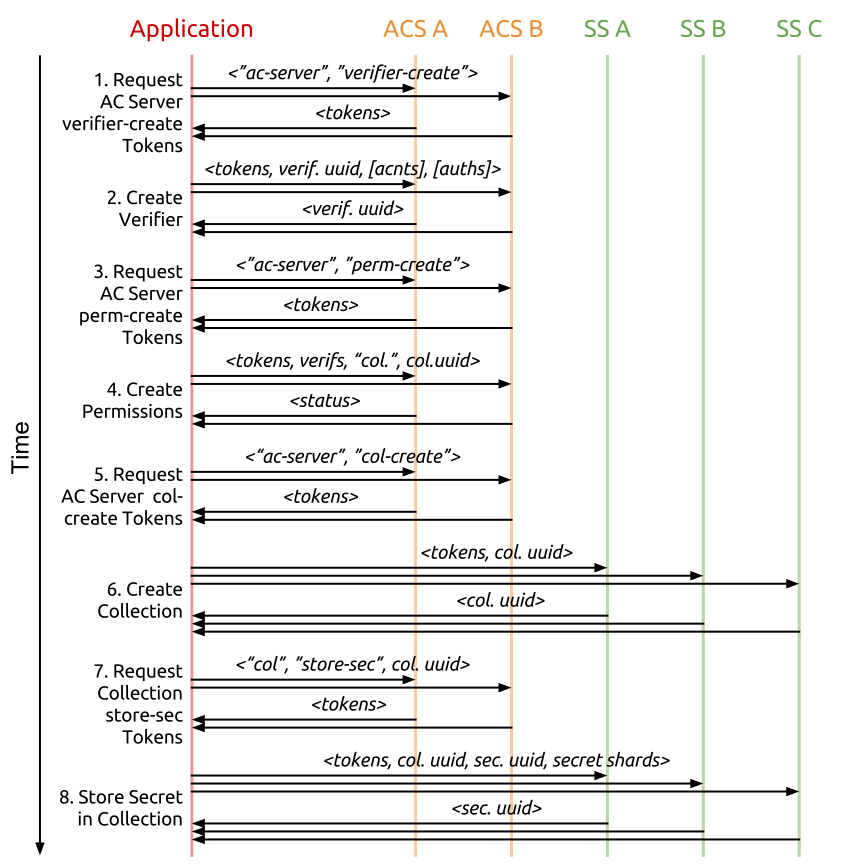
\includegraphics[width=\textwidth]{./figs/out/Tutamen-Op-Store.pdf}
    \caption{Storing a New Secret}
    \label{fig:tutamen:ops:store}
  \end{subfigure}
  ~
  \begin{subfigure}[t]{0.48\textwidth}
    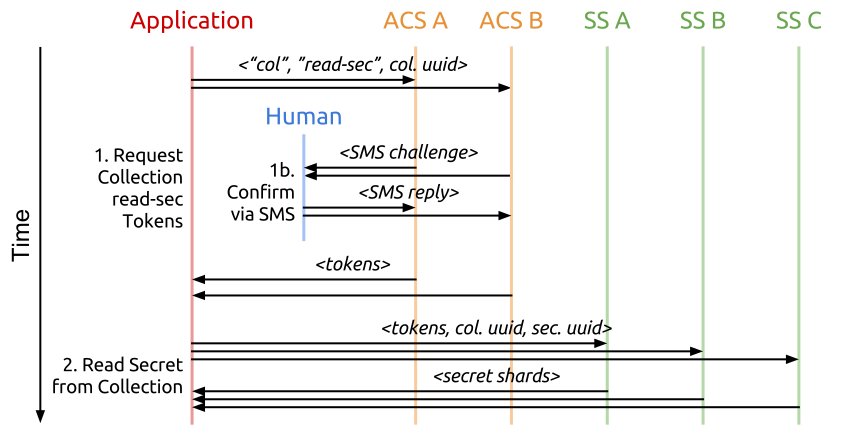
\includegraphics[width=\textwidth]{./figs/out/Tutamen-Op-Fetch.pdf}
    \caption{Retrieving an Existing Secret (w/ SMS Auth)}
    \label{fig:tutamen:ops:fetch}
  \end{subfigure}
  \caption{Tutamen Operations}
  \label{fig:tutamen:ops}
\end{figure}

An example of the steps taken by an application to store and then
retrieve a secret via Tutamen is useful for illustrating the
interaction of the various components of the Tutamen platform. In this
example, the Tutamen application is using three storage servers and
two access control servers as shown in
Figure~\ref{fig:tutamen:systemdistributed}. The application has also
already bootstrapped an account and client (i.e., it previously
contacted the AC servers with a request to create a new account and
associated client).

Figure~\ref{fig:tutamen:ops:store} shows the steps required to create
a new collection and store a secret within it. This diagram assumes
the application has already sharded its secret into three parts -- one
per server.\footnote{Omitted from this diagram is the process of
  creating verifiers and permissions groups for the collection
  verifier itself. These permissions groups are necessary to control
  who can read, modify, or delete the corresponding verifier after
  creation. The process for creating said structures is similar to the
  process of creating the collection-related verifier and permissions
  group shown. To avoid the infinite recursion of needing verifiers
  for each verifier, it is possible for a verifier to be associated
  with a permissions group in which it is itself a member (i.e., a
  verifier can enforce its own access control specification).}

Figure~\ref{fig:tutamen:ops:fetch} shows the steps required to
retrieve an existing secret. This diagram also assumes that the secret
in question has an SMS authenticator associated with it, requiring a
user to provide a response to an SMS challenge approving access to the
secret.

\section{Tutamen Implementation}
\label{chap:tutamen:imp}

Tutamen reference implementations exist for the storage server, access
control server, client libraries, and several applications. These
implementation allow for the testing of the Tutamen platform and
concepts. The details of these implementations are discussed below.

\subsection{Server Implementation}
\label{chap:tutamen:imp:server}

The Tutamen server implementations expose RESTful
interfaces~\cite{fielding2000} for both the access control and storage
server APIs. These interfaces both accepts and responds using
JSON~\cite{json} messages over the HTTPS protocol. The full access
control server API specification as well as the API reference
implementation source code is available
at~\cite{src-tutamen-apiaccesscontrol}. Likewise, the storage server
API specification and source code can be found
at~\cite{src-tutamen-apistorage}. Both implementations are freely
available under the terms of the AGPLv3. The prototype servers are
written in Python 3 using the Flask web
framework~\cite{python-flask}. Both servers are designed to be served
via WSGI~\cite{pep3333} using the Apache HTTP Server~\cite{apache} for
TLS termination and client-certificate verification.

Both Tutamen servers rely on a shared \texttt{pytutamen-server} python
library for the implementation of their core logic. The
\texttt{pytutamen-server} source is available
at~\cite{src-tutamen-pytutamenserver} under the terms of the
LGPLv3. This library leverages the Redis~\cite{redis} key-value store
for persistent storage. The Tutamen reference implementation adopts
the JSON Web Signature (JWS)~\cite{rfc7515} and JSON Web Token
(JWT)~\cite{rfc7519} specifications for exchanging cryptographically
authenticated tokens between Tutamen applications, access control
servers, and storage servers. The implementation leverages the
pyjwt~\cite{pyjwt} library for JWS and JWT support. These tokens are
attached to subsequent requests using a \texttt{tutamen-tokens} header
field. The \texttt{pytutamen-server} library relies on the Python
Cryptography~\cite{python-cryptography} library for CA-related
certificate provisioning duties.

The access control servers expose a pluggable authenticator interface
through which end users and other developers may add custom
authentication functionality. This interface is similar in purpose to
previous pluggable authentication interfaces such as
PAM~\cite{samar1996}. The Tutamen authenticator interface is primarily
designed for providing authentication checks beyond the TLS client
certificate authentication the access control server automatically
performs on every request for the purpose of associating each request
with a specific client and account. The reference AC server
implementation includes an example SMS authenticator module that
allows users to approve Tutamen token requests via SMS text message
using the Twilio~\cite{twilio} messaging platform. Additional
authenticator modules might include support for only allowing requests
during certain times of day or from specific network addresses. Each
authenticator plugin is provided with both a set of per-instance
configuration data (e.g., to whom an SMS message gets sent for
approval) as well as all of the details of a specific token request
including both the IDs and metadata associated with the requesting
account and client (e.g., from which information such as originating
IP address or time of day can be extracted).

\subsection{Client Implementation}
\label{chap:tutamen:imp:client}

In addition to the server and authenticator implementations, there are
also reference Tutamen client libraries for both
Python~\cite{src-tutamen-pytutamen} and
Go~\cite{src-tutamen-go}.\footnote{The Go client library was created
  by Matthew Monaco.} The Python client library services as the basis
for the reference Tutamen CLI utility. This utility allows users to
directly store/retrieve secrets from Tutamen storage servers and to
control secret sharing and access control rules on Tutamen AC
servers. The CLI is useful for managing Tutamen objects even in cases
where other applications (e.g., those discussed in
Section~\ref{chap:tutamen:imp:apps}) are set up to interface directly
with the Tutamen platform. As discussed in Chapter~\ref{chap:apps}, it
is not necessary for every SSaaS application to implement all SSaaS
functionality. Instead, an application might leverage only the
necessary Tutamen commands to perform secret storage and retrieval,
leaving the task of managing the sharing of Tutamen-stored secrets to
the CLI or to another dedicated management application.

\subsection{Applications}
\label{chap:tutamen:imp:apps}

Tutamen is designed to support a wide range of applications.  The
reference Tutamen design includes a set of reference applications for
the purpose of demonstrating the value derived from using a secure
storage system such as Tutamen. These applications all leverage
Tutamen's flexibility to achieve functionality that would have been
difficult or impossible to achieve without using an SSaaS system like
Tutamen.

\subsubsection{Block Device Encryption}

As discussed in Chapters~\ref{chap:challenges} and~\ref{chap:apps},
block device encryption systems are a popular means of protecting the
data stored on computing systems in the event that the system is lost,
stolen, or otherwise physically compromised.  Block-level encryption
systems such as dm-crypt~\cite{dm-crypt} (generally coupled with a
Linux Unified Key Setup (LUKS)~\cite{luks} container) or the
QEMU~\cite{qemu} qcow2 encryption system provide methods for securing
the data stored on laptops, desktops, and VMs. Such systems
traditionally bootstrap security by requiring the user to enter a
password at boot-time to unlock a locally stored encryption key which
is then used to decrypt the block device in question. Unfortunately,
the ``human-at-keyboard'' security root make such systems difficult or
impossible to use atop headless servers or in other situations where
no human can be expected to be present at boot-time. Interfacing
Tutamen with such applications overcomes this barrier.

In order to add Tutamen support to dm-crypt/LUKS, it was necessary to
create a Tutamen-aware implementation~\cite{src-tutamen-askpassword}
of the \texttt{systemd} Password Agent
Specification~\cite{systemd-passwordagents}.\footnote{Matt Monaco is
  primarily responsible for the Tutamen dm-crypt integration.}  This
specification is used by the LUKS/dm-crypt \texttt{cryptsetup} utility
to request the necessary decryption secret. At boot-time,
\texttt{cryptsetup} will send out a request for this secret. Normally
this triggers a ``human-at-keyboard'' prompt for a boot passphrase. A
Tutamen-aware password agent can instead respond to such requests by
retrieving the necessary decryption secret from a Tutamen storage
server (after first retrieving the necessary tokens from the
corresponding Tutamen AC server). In order to support Tutamen use in a
pre-boot environment, several modifications had to be made to the
\texttt{initrd} creation process to add Tutamen networking support,
the necessary Tutamen client TLS key pair, and a config file
specifying which Tutamen servers to use and the UUIDs of the relevant
Tutamen collection and secrets.

In addition to dm-crypt/LUKS support, the Tutamen reference
implementation also supports QEMU's \texttt{qcow2} VM disk encryption
system~\cite{src-qemu-tutamen}. Similar to the dm-crypt setup, QEMU
normally requires the user to provide the encryption key via the QEMU
console when a VM launches. A SSaaS-backed QEMU encryption system
replaces this ``human-at-keyboard'' process with Tutamen-based secret
retrieval. In addition, QEMU currently requires the user to provide
the full encryption key, not just a passphrase to unlock a pre-stored
key~\cite{berrange-qemucrypto}. This has negative security
repercussions in the common case where users pick short password-like
keys. Using Tutamen, users can overcome this barrier since Tutamen
servers have no qualms about needing to store or remember sufficiently
long encryption keys. This system thus increases the security and ease
of use of QEMU's \texttt{qcow2} encryption.

Using these setups, a user is able to boot servers and VM images with
encrypted disks without requiring a human to be physically present at
the machine. In cases where they still desires human approval of the
boot process, the user can leverage the SMS authenticator module to
get an on-demand confirmation from a designated human as a
prerequisite to Tutamen releasing the correct key. This allows the
user to gain the same level of human-in-the-loop security provided by
a typed passphrase, but without actually requiring a human to go to
the datacenter to type one in. In situations where one doesn't desire
a human-in-the-loop at all, Tutamen-backed system could support
automating the approval process via the use of time-of-day and
IP-source authenticators.

\subsubsection{Encrypted Cloud File Locker}

Cloud-based file lockers such as Dropbox~\cite{dropbox} are extremely
popular today. Unfortunately, these systems require users to trust the
cloud provider with full access to their (generally unencrypted)
data. Users wishing to overcome this deficiency can optionally encrypt
all of their data on the client before syncing it to the file locker
provider, but as discussed in Chapter~\ref{chap:challenges}, doing so
does not generally interact well with such services' sharing and
multi-device use cases.

Tutamen provides a solution to this problem by offering a secure
key-sharing mechanism. Instead of manually distributing or sharing
encryption keys, the user can store their key as a Tutamen secret and
leverage Tutamen's access control features to share the secret with
the accounts of their friends. This entire process could even be
automated such that when a user shares a file via Dropbox, the
corresponding encryption key is automatically shared via Tutamen.

Toward this end, the Tutamen reference implementation includes
FuseBox: an alternate Dropbox client that performs client-side
encryption of all Dropbox files, storing the corresponding encryption
keys on the reference Tutamen server~\cite{fusebox}.\footnote{Taylor
  Andrews is primarily responsible for the Tutamen FuseBox
  implementation.} FuseBox achieves goals similar to those achieved
by~\cite{goh2003}, but without requiring out-of-band key
management. Similar to other file-system-level encryption
systems~\cite{blaze1993, Cattaneo2001, halcrow}, FuseBox provides
transparent file encryption to end users. In order to avoid the
storage space and security challenges presented by locally caching all
Dropbox data (i.e., the operation mode for the official Dropbox
client), FuseBox uses AES~\cite{daemen1999, nist2001} in a stream
cipher mode to transparently stream and encrypt data to/from
Dropbox's servers on demand.

Since FuseBox leverages Tutamen to store each per-file encryption key,
it becomes possible to share an encrypted file via Dropbox, share its
encryption key via Tutamen, and achieve the same level of
functionality traditional Dropbox users have without having to expose
one's data to Dropbox. While the key sharing process in FuseBox is not
yet directly synced with Dropbox's file sharing system, the Tutamen
CLI can be used to quickly share the encryption keys between users. In
this manner, users can use FuseBox to store and share encrypted files
with nearly the same ease with which they might use the traditional
unencrypted Dropbox client. By leveraging Tutamen, FuseBox also gains
the ability to remotely revoke file access, e.g., in the case a device
is lost or stolen, similar to systems such
as~\cite{geambasu2011}. While FuseBox does not currently authenticate
data, such support could be add to FuseBox's streaming architecture
using techniques such as those described
at~\cite{McGrew2005}. FuseBox, via Tutamen's distributed operation
mode, also avoids the sharing pitfalls associated many existing
``secure cloud storage'' providers~\cite{wilson2014} by avoiding
reliance on a single trusted party or CA to facilitate sharing
operations.

\subsection{Other}

Since the reference Tutamen-backed \texttt{ask-password}
port~\cite{src-tutamen-askpassword} speaks the standard
\texttt{systemd} Password Agent protocol, it can also be used to
provide Tutamen-backed passphrase storage to any applications
leveraging this protocol. This includes OpenVPN and various password
storage utilities. As such, the Tutamen-passed \texttt{systemd}
password agent is potentially useful in a wide range of situations
beyond just full disk encryption. The experience of integrating the
systemd password agent with Tutamen also suggests that Tutamen would
provide a useful backend for a variety of other ``agent'' protocols
(e.g.,~\cite{cox2002, ylonen1996}), adding support for the kinds of
SSH key management applications discussed in Chapter~\ref{chap:apps}.

\section{Security and Trust in Tutamen}
\label{chap:tutamen:trust}

One of Tutamen's primary design goals is its ability to support a wide
range of security and trust requirements. It achieves this goal
through its support for both centralized and distributed operation as
well as though its support for a range of authentication mechanisms.

\subsection{Security of Individual Servers}

The security of each individual access control server rests on several
requirements. Failure to uphold these requirements will result in the
failure of any security guarantees provided by the AC server.

\begin{packed_desc}
\item[Certificate Authority Role:] Each access control server acts as
  a CA delegated with issuing and verifying client certificates. Thus,
  each AC server must store its CA keys in a secure manner and
  faithfully verify the certificate presented by each client
  connection.
\item[Token Issuance and Verification:] Each access control server is
  responsible for verifying the access control requirements bound to
  specific object/permission combinations, issuing signed tokens
  attesting to such verification, and verifying the signatures of the
  tokens it receives from clients wishing to operate on access control
  objects. Thus, each AC server must store its private token signing
  key in a secure manner and faithfully verify both the access control
  requirements governing specific token requests as well as the
  signatures on all incoming tokens.
\end{packed_desc}

The storage servers must uphold the following security
requirements. Failure to do so results in a failure of the security of
the storage server.

\begin{packed_desc}
\item[Token Verification:] Each storage server must securely (via
  HTTPS) obtain the public token signing key from each AC server
  delegated with providing access control for a given storage
  object. The storage server must then use these keys to faithfully
  verify the signatures on all tokens it receives. Assuming the token
  signature is valid, the storage server must faithfully enforce the
  claims asserted in a given token by only allowing actions granted by
  the permission contained in the token on the object the token
  identifies prior to the expiration time specified by the token.
\item[Secure Storage:] Each storage server must take steps to store
  user-provided secrets in a secure manner, releasing them only to
  requests accompanied by the requisite number of valid tokens
  granting such release.
\end{packed_desc}

Since the tokens the storage server must verify are provided by the AC
servers, the security of the storage server with respect to a given
collection is dependent on the security of any designated AC servers
associated with said collection. If these AC servers are insecure, the
objects that delegate access to them will also be insecure.

\subsection{Security of Multiple Servers}

Unlike existing secret management systems~\cite{vault, confidant,
  keywhiz}, the Tutamen architecture is capable of remaining secure
even when individual storage or access control servers fail to meet
their security requirements. Such failures may result from any of the
violations discussed in Chapter~\ref{chap:trust} including physical
server compromise, software bugs, malicious intent, incompetence or
legal obligations (e.g., being forced to turn over stored secrets in
response to legal or political pressure).

To work around security failures of individual servers, Tutamen
applications can leverage Tutamen's distributed operation modes. In
these modes, the security of the system as a whole is diffused, no
longer relying on the security of any specific access control or
storage server in order to keep an application's secrets secure. As
described in Section~\ref{chap:tutamen:arch:distributed}, each
application can distribute both secret storage and access control
delegations using $n$ choose $k$ schemes. In such setups, the
difference between $n$ and $k$ dictates the degree of redundancy
inherent in the system while the value of $k$ dictates the degree by
which a Tutamen application can withstand security failures. For
example, an application which chooses to shard its secrets across six
storage servers where any three shards are sufficient to recreate the
secret ($n=6$, $k=3$) will continue to remain secure even if two
(i.e. $k-1$) of the storage servers fail to meet their security
obligations. The system will also remain available even if three
(i.e. $n-k$) of the servers fail to return secret shards. Similarly,
if each secret shard delegates six possible AC servers, tokens from
three of which are required to grant secret access, the application
can withstand the failure of two AC servers to uphold their security
guarantees and the failure of three AC servers to return tokens.

\subsection{Trust Model}

Trust in Tutamen follows from the security models of both individual
Tutamen servers and of the distributed Tutamen deployment
architectures. If a Tutamen application is leveraging only a single
storage and AC server, the application is placing a high degree of
trust in both servers (and by proxy, the operators of both
servers). This level of trust may be appropriate for some use cases
(e.g., when a user is operating their own Tutamen's servers), but is
inappropriate in many other cases (e.g., when using third party hosted
Tutamen servers). Fortunately, Tutamen allows applications to avoid
placing a high degree of trust in any single server by leveraging
multiple servers and picking $k$ and $n$ in a manner commensurate with
the degree to which each server is trusted.

Beyond minimizing the amount of trust placed in each individual
Tutamen server by leveraging multiple servers, Tutamen also follows
the SSaaS pattern of aligning trust with economic incentives (see
\S~\ref{chap:ssaas:economics}). The Tutamen protocol is standardized
and designed to support a range of interchangeable ACS and SS
providers. Such a design allows for the development of a Tutamen
server marketplace where both ACS and SS providers can compete against
each other on the basis of trustworthiness, features (e.g., what types
of authenticators they support), and cost. In such an ecosystem,
Tutamen service providers who fail to uphold the Tutamen security
requirements on their servers will suffer a negative economic effect,
disincentivizing such behavior. It is also likely that storage
providers who take additional steps to protect the secrets they store
(e.g., by using systems such as Trusted Platform Modules (TPMs) to
encrypt the secrets they hold and harden server security) would be
able to command a higher price in the marketplace, incentivizing such
best practices.

Thus, unlike other third party cloud services where trustworthiness
and economic incentives are in direct competition (as is the case on
many ``free'' third part services that depend on selling user data in
order to generate revenue), Tutamen encourages a system where economic
incentives are well aligned with user trust. That fact, coupled with
the high degree of control over third party trust Tutamen grants to
each application by allowing each application to select how many
servers to diffuse trust across, make Tutamen a robust system in the
face of both security and trustworthiness failures. Such robustness is
a critical component of the SSaaS model.

\section{Tutamen Evaluation}
\label{chap:tutamen:eval}

\begin{figure}[!t]
  \centering
  \begin{subfigure}[t]{0.48\textwidth}
    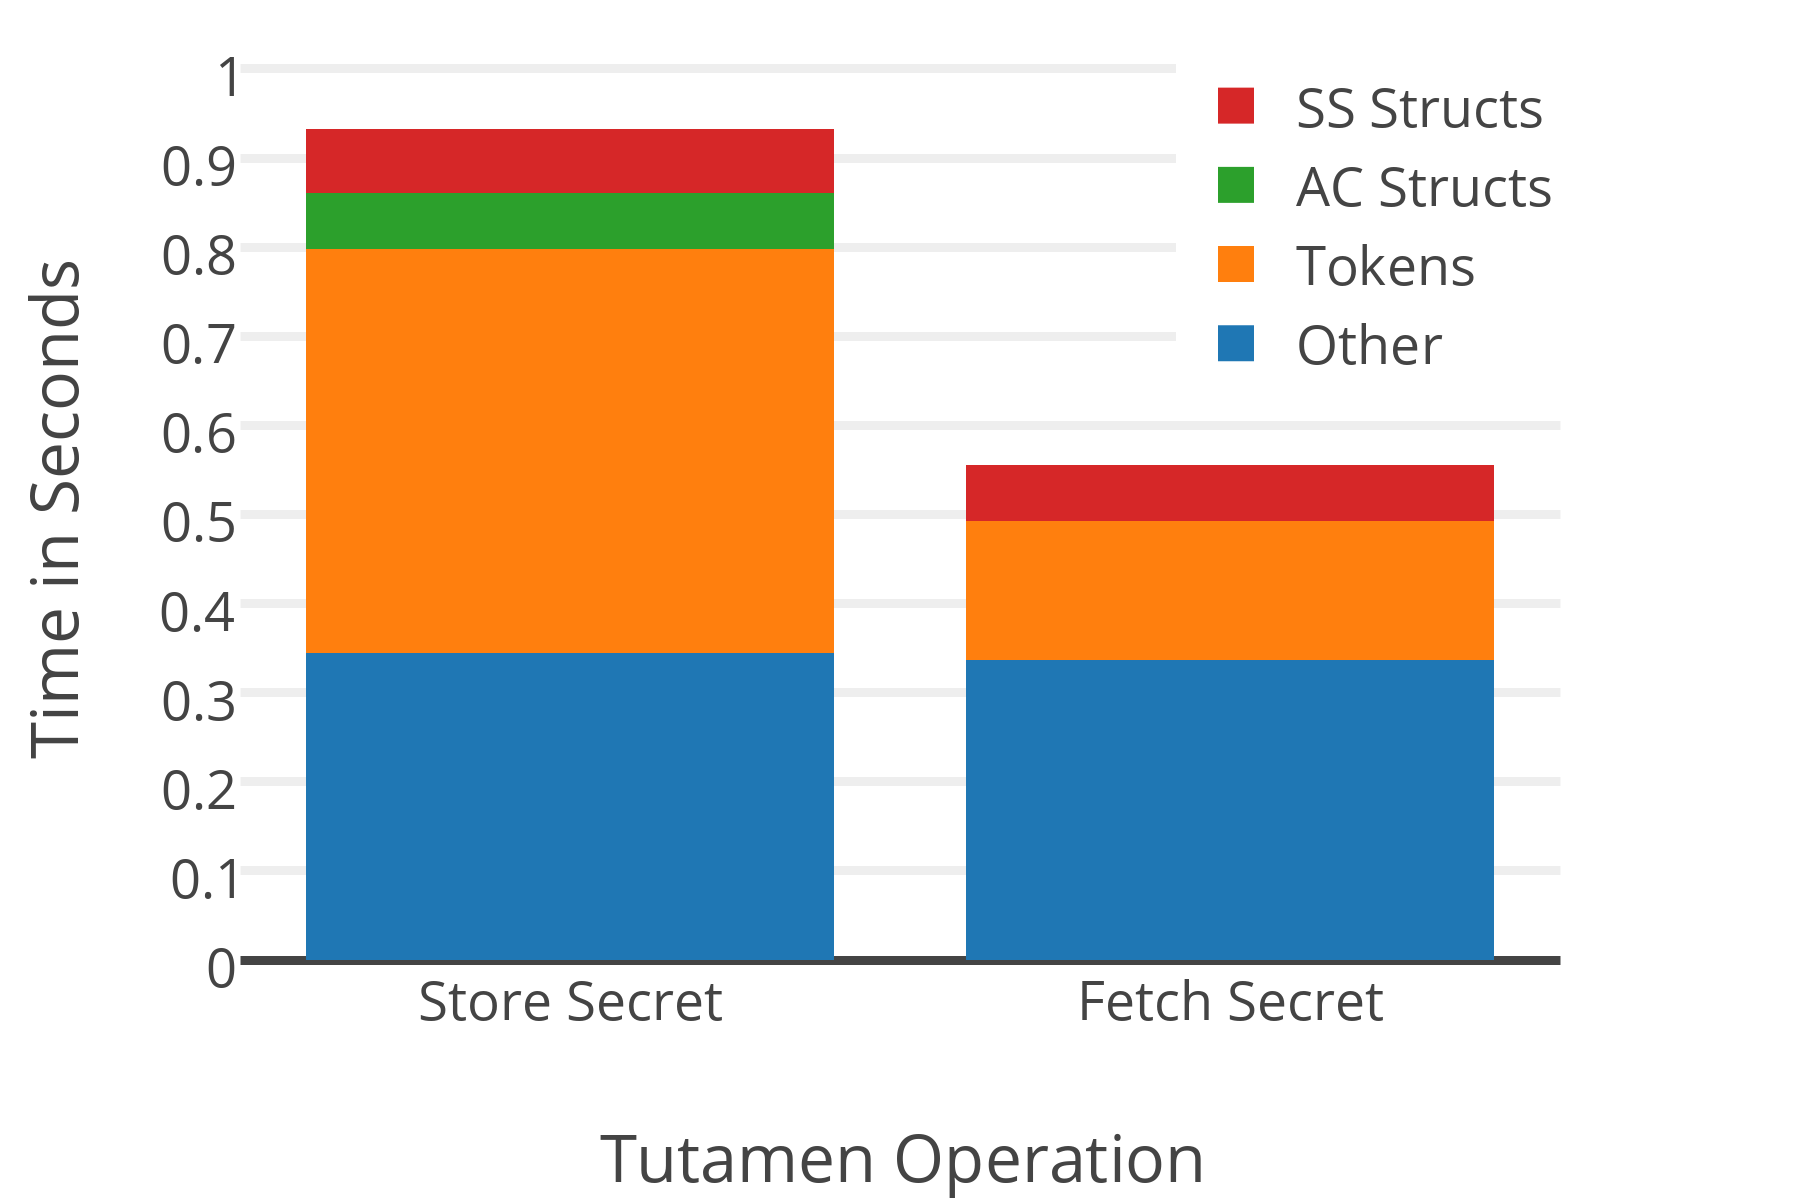
\includegraphics[width=\columnwidth]{./figs/pre/Tutamen-Chart-Timings.png}
    \caption{Timings for Tutamen Operations}
    \label{fig:tutamen:charts:timings}
  \end{subfigure}
  ~
  \begin{subfigure}[t]{0.48\textwidth}
    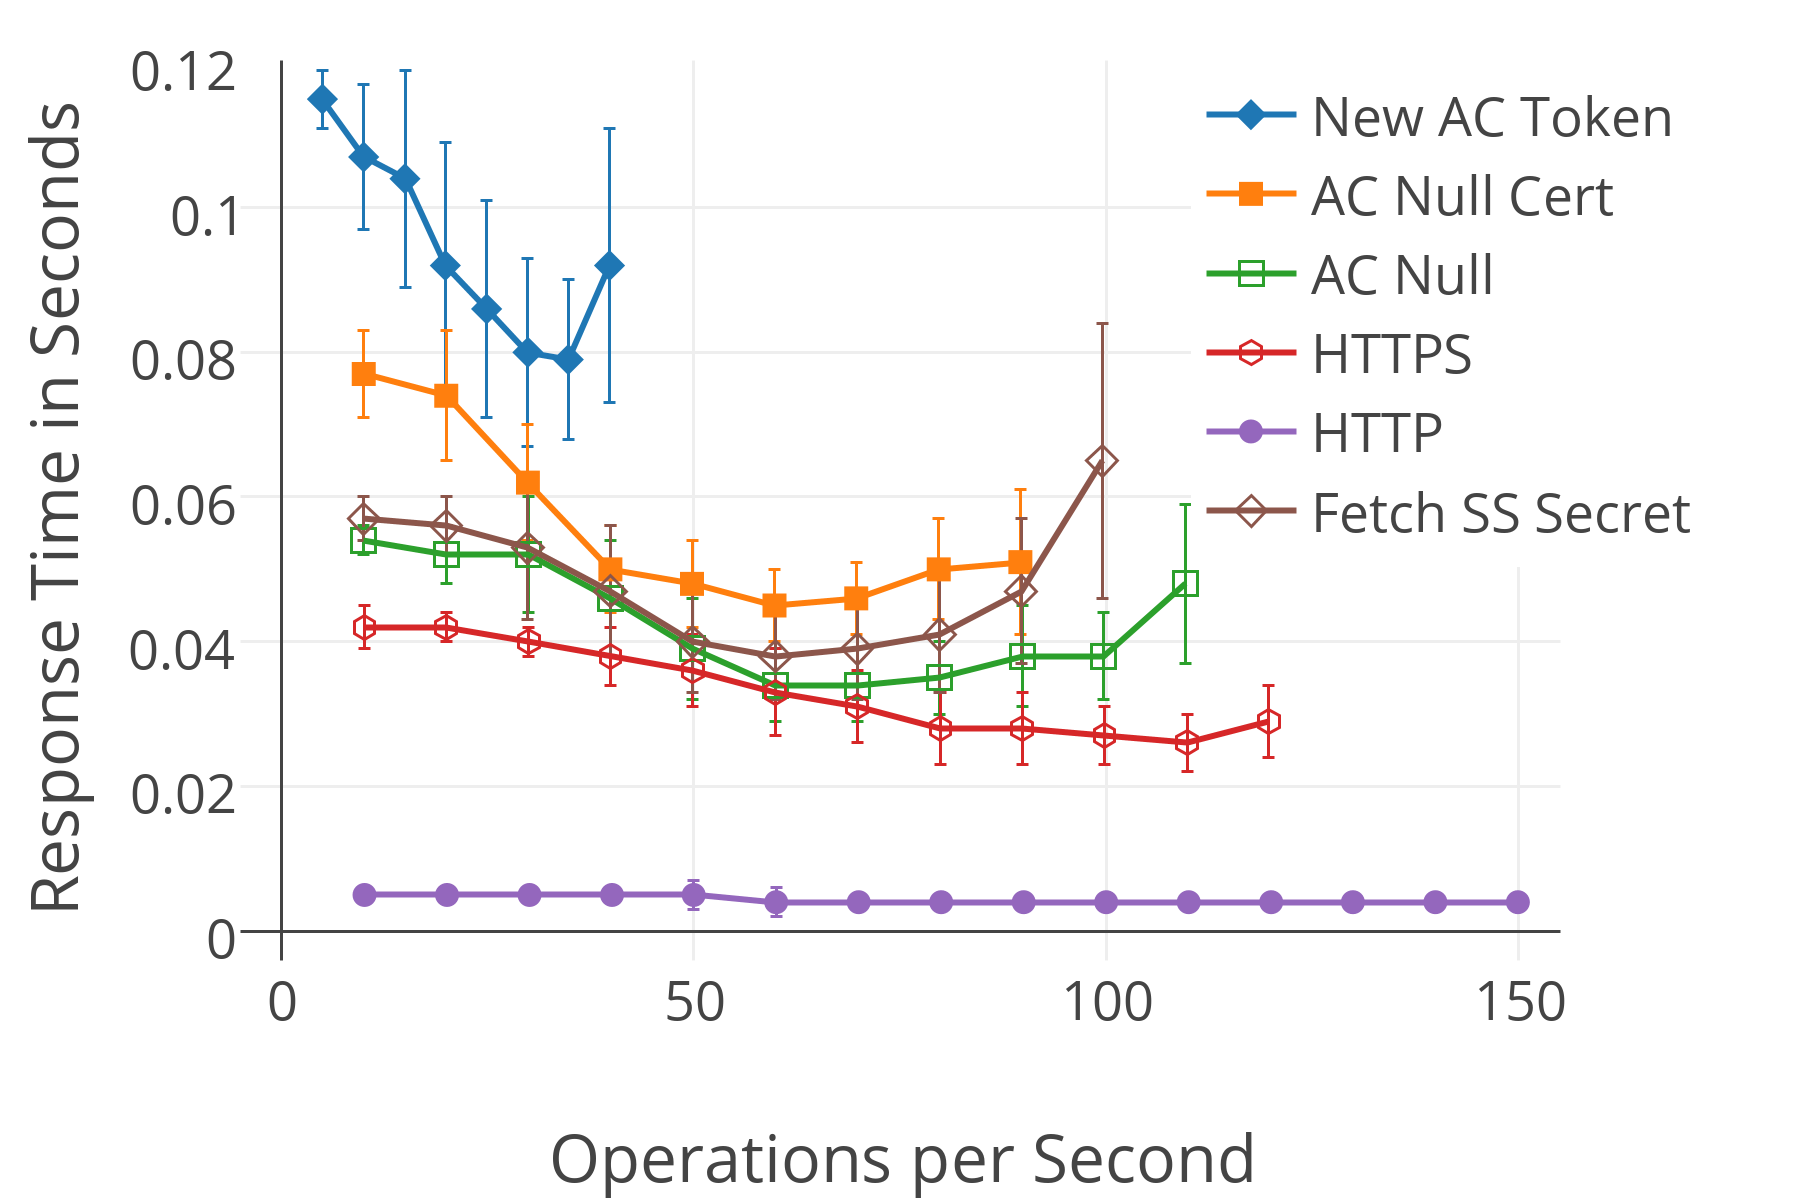
\includegraphics[width=\columnwidth]{./figs/pre/Tutamen-Chart-IOPS.png}
    \caption{Throughput vs Latency Curves}
    \label{fig:tutamen:charts:iops}
  \end{subfigure}
  \caption{Tutamen Performance}
  \label{fig:tutamen:charts}
\end{figure}

The Tutamen reference implementation has been evaluated in a variety
of scenarios using the applications described in
\S~\ref{chap:tutamen:imp:apps}. These scenarios have proven Tutamen's
usefulness as an enabler of previously unattainable
functionally. While Tutamen is still a prototype, it provides a
well-designed architecture capable of supporting a wide range of
practical secret storage applications. The use of strong encryption in
these applications would be difficult (or at least burdensome on the
end user) to realize without a system such as Tutamen.

Since the Tutamen reference implementation has not yet been optimized
for performance, it is more useful to compare relative computational
loads than the absolute speed of the Tutamen system. Such a comparison
can be achieved by profiling the amount of time the Tutamen CLI
utility spends performing various parts of each of these two Tutamen
operations. Figure~\ref{fig:tutamen:charts:timings} shows the time
required to complete two of the most common Tutamen operations:
storing a new secret and retrieving a previously stored secret. In
both operations, the bulk of the server-related run time is spent
requesting and retrieving the authorization tokens required to
complete the associated operations. In the secret creation case, five
tokens are required. In the secret read case, only a single token is
required. The remainder of the server-related time is spent either
creating AC and storage data structures (as in the store secret case),
or reading existing data structures (as in the retrieve secret
case). The ``other'' time is spent reading the Tutamen config files,
loading the necessary client certificates, and dealing with the
overhead required to interpret the python-based CLI.

It is not unexpected that a Tutamen client must spend the bulk of its
time requesting tokens and waiting for them to be approved -- token
verification is the primary role the access control server must
perform, and depending on the complexity of the verifiers associated
with the permission the token is requesting, verification can be a
fairly complex task. These measurements were obtained using a simple
verifier that only required client membership in a specific
account. Verifiers that include human-in-the-loop authenticators
(e.g., SMS approval) would increase the token turnaround time by the
amount of time the human requires to provide approval. Thus, it is
important that Tutamen applications treat token approval as an
operation that can take anywhere from under a second to human-scale
times (e.g., 10s of seconds). To help alleviate these waits on
applications that must perform a high number of Tutamen requests,
Tutamen tokens may be reused up until their expiration time. Thus, it
is possible for an application to request a long-lived token and to
reuse this token to access multiple secrets within the collection to
which the token grants read access.

Figure~\ref{fig:tutamen:charts:iops} shows the request rate vs
response time (with standard deviations) of a token request operation,
two ``null'' AC API operations (one that sends and verifies the client
TLS certificate and one that does not), and a fetch secret
operation. Raw Apache HTTPS and HTTP curves are also shown for
comparison. As these curves show, token verification for the reference
server tops out at around 40 requests/second (rps) on a modest server
(2-core, 4GB VM running atop 2011-era Intel Xeon hardware). The null
AC API operation with client certificates tops out around 90 rps, and
the null operation without client certificates tops out at about 110
rps. Raw HTTPS tops out around 120 rps. HTTP topped out around 5000
rps (curve truncated for viewability). The current server setup is
thus primarily limited by the crypto overhead required to serve the
application and verify client certificates using TLS. Token
verification itself also incurs additional computational requirements,
including cryptographic signing operations, but is well within the
order of magnitude of the underlying server limits. Secret retrieval
(after acquiring a token) is relatively quick, topping out at around
100 rps.

While these levels of performance would not likely meet the
requirements of a production-level Tutamen AC server, they have been
perfectly adequate for supporting the Tutamen applications discussed
in \S~\ref{chap:tutamen:imp:apps}. Since most of these Tutamen
applications require only a single Tutamen secret retrieval at
relatively rare rates (e.g., once per server reboot or once per file
open), the 40+ requests per second the AC server can provide have been
more than adequate for their needs. The Tutamen reference servers are
also designed to be horizontally scalable (e.g., by spinning up
multiple load-balanced servers that share a common database). That
scalability, coupled with future performance-related code
optimization, suggests that the Tutamen server infrastructure can be
adopted to meet the needs of larger installations with only moderate
effort.

%%  LocalWords:  HashiCorp's Lyft's Keywhiz TPMs QEMU's Xeon Tutamen
%%  LocalWords:  viewability Custos ACS HTTPS CSR CSRs authenticators
%%  LocalWords:  Authenticators verifiers authenticator DoS AGPLv JWS
%%  LocalWords:  pytutamen LGPLv Redis JWT pyjwt tutamen SMS Twilio
%%  LocalWords:  Auth Tutamen's dm QEMU qcow systemd cryptsetup SSaaS
%%  LocalWords:  initrd FuseBox FuseBox's OpenVPN Custos's SSP
%%  LocalWords:  passphrase
